\chapter{Rozwiązania}


\section*{Rozdział 2}
\label{sol:2}

\subsection*{Ćwiczenie 2.1}
\label{sol:2.1}

Wynikiem tego wyrażenia jest \texttt{true}. Można je rozłożyć na czynniki:

\begin{verbatim} 
(false || true) && !(false && true)
\end{verbatim}

\begin{verbatim} 
true && !false
\end{verbatim}

\begin{verbatim} 
true
\end{verbatim}
      
Mam nadzieję, że zauważyłeś, że wyrażenie \texttt{"zielona" != "trawa"} jest prawdziwe. Oczywiście trawa może być zielona, ale to są dwa różne słowa.

\subsection*{Ćwiczenie 2.2}
\label{sol:2.2}

\begin{verbatim} 
var wynik = 1;
var licznik = 0;
while (licznik < 10) {
  wynik = wynik * 2;
  licznik = licznik + 1;
}
show(wynik);
\end{verbatim}
      
Licznik równie dobrze mógłby mieć wartość początkową \texttt{1} i wówczas test wyglądałby tak: \texttt{<= 10}. Jednak są powody, które poznasz później, aby przyzwyczaić się do liczenia od zera.

      
Oczywiście Twoje rozwiązanie nie musi być identyczne z moim. Powinno tylko działać. Jeśli Twoje rozwiązanie różni się od mojego, postaraj się dokładnie zrozumieć także mój kod.

\subsection*{Ćwiczenie 2.3}
\label{sol:2.3}

\begin{verbatim} 
var linia = "";
var licznik = 0;
while (licznik < 10) {
  linia = linia + "#";
  print(linia);
  licznik = licznik + 1;
}
\end{verbatim}

\subsection*{Ćwiczenie 2.4}
\label{sol:2.4}

\begin{verbatim} 
var wynik = 1;
for (var licznik = 0; licznik < 10; licznik = licznik + 1)
  wynik = wynik * 2;
show(wynik);
\end{verbatim}
      
Zwróć uwagę, że nawet mimo braku znaku \texttt{\{} oznaczającego początek bloku, instrukcja w pętli i tak została wcięta, aby było jasne, że należy do wiersza kodu znajdującego się nad nią.

      
\begin{verbatim} 
var linia = "";
for (var licznik = 0; licznik < 10; licznik = licznik + 1) {
  linia = linia + "#";
  print(linia);
}
\end{verbatim}

\subsection*{Ćwiczenie 2.5}
\label{sol:2.5}

\begin{verbatim} 
var odpowiedz = prompt("Hej, Ty! Ile wynosi 2 + 2?", "");
if (odpowiedz == "4")
  alert("Jesteś genialny.");
else if (odpowiedz == "3" || odpowiedz == "5")
  alert("Prawie!");
else
  alert("Żal mi Ciebie.");
\end{verbatim}

\subsection*{Ćwiczenie 2.6}
\label{sol:2.6}

\begin{verbatim} 
var odpowiedz;
while (true) {
  odpowiedz = prompt("Hej, Ty! Ile wynosi 2 + 2?", "");
  if (odpowiedz == "4") {
    alert("Jesteś genialny.");
    break;
  }
  else if (odpowiedz == "3" || odpowiedz == "5") {
    alert("Prawie!");
  }
  else {
    alert("Żal mi Ciebie.");
  }
}
\end{verbatim}
      
Ponieważ treść pierwszej instrukcji \texttt{if} zawiera teraz dwie instrukcje, dodałem klamry. Jest to kwestia gustu. Łańcuchy instrukcji \texttt{if}/\texttt{else}, w których niektóre klauzule zawierają bloki, a inne pojedyncze instrukcje jak dla mnie wyglądają dziwnie, ale może Ty będziesz miał inne zdanie na ten temat.

Oto inne rozwiązanie, bez użycia instrukcji \texttt{break} i może trochę bardziej eleganckie:
      
\begin{verbatim} 
var wartosc = null;
while (wartosc != "4") {
  wartosc = prompt("Hej, Ty! Ile wynosi 2 + 2?", "");
  if (wartosc == "4")
    alert("Jesteś genialny.");
  else if (wartosc == "3" || wartosc == "5")
    alert("Prawie!");
  else
    alert("Żal mi Ciebie.");
}
\end{verbatim}


\section*{Rozdział 3}
\label{sol:3}

\subsection*{Ćwiczenie 3.1}
\label{sol:3.1}
      
\begin{verbatim} 
function absolute(number) {
  if (number < 0)
    return -number;
  else
    return number;
}

show(absolute(-144));
\end{verbatim}
    
\subsection*{Ćwiczenie 3.2}
\label{sol:3.2}
     
\begin{verbatim} 
function greaterThan(x) {
  return function(y) {
    return y > x;
  };
}

var greaterThanTen = greaterThan(10);
show(greaterThanTen(9));
 \end{verbatim}
 

\section*{Rozdział 4}
\label{sol:4}
    
\subsection*{Ćwiczenie 4.1}
\label{sol:4.1}

Zadanie to można wykonać zapisując zawartość zbioru jako własności obiektu. Dodawanie imion polegałoby na zdefiniowaniu własności o takich nazwach i dowolnych wartościach. Usuwanie imion polegałoby na kasowaniu odpowiadających im własności. Za pomocą operatora \texttt{in} można natomiast sprawdzać, czy wybrane imię znajduje się już w zbiorze \footnote{Podejście to ma kilka subtelnych wad, które zostaną omówione w \hyperref[chap:8]{rozdziale 8}. W~tym rozdziale wystarczy to, co jest.}.
      
\begin{verbatim} 
var set = {"Spot": true};
// Dodanie White Fang do zbioru
set["White Fang"] = true;
// Usunięcie Spot
delete set["Spot"];
// Sprawdzenie czy "Asoka" znajduje się w zbiorze
show("Asoka" in set);
 \end{verbatim}
    
  
\subsection*{Ćwiczenie 4.2}
\label{sol:4.2}
      
\begin{verbatim} 
function range(upto) {
  var result = [];
  for (var i = 0; i <= upto; i++)
    result[i] = i;
  return result;
}
show(range(4));
 \end{verbatim}
      
Zamiast zmienną pętlową nazywać \texttt{counter} albo \texttt{current}, jak było do tej pory, tym razem nadałem jej nazwę \texttt{i}. Stosowanie jednoliterowych nazw, zazwyczaj \texttt{i}, \texttt{j} lub \texttt{k}, dla zmiennych pętlowych jest szeroko przyjętym zwyczajem wśród programistów. Źródeł jego powstania należy upatrywać przede wszystkim w lenistwie: każdy woli wpisać jedną literę zamiast siedmiu, a~nazwy typu \texttt{counter} albo \texttt{current} i tak niewiele wyjaśniają, do czego dana zmienna służy.

      
Jeśli jednak w programie znajdzie się zbyt dużo jednoliterowych nazw zmiennych, to zrozumienie sposobu jego działania może stać się strasznie trudne. We własnych programach staram się tak krótkich nazw używać tylko w kilku typowych przypadkach. Należą do nich także niezbyt rozbudowane pętle. Jeśli pętla zawiera inną pętlę, która również ma zmienną o nazwie \texttt{i}, wewnętrzna pętla zmodyfikuje zmienną używaną przez zewnętrzną pętlę i nastąpi wielka awaria. W wewnętrznej pętli można by było zatem użyć nazwy \texttt{j}, ale ogólnie rzecz biorąc przyjmuje się, że jeśli pętla jest rozbudowana, powinno się użyć jakiejś znaczącej nazwy zmiennej, aby łatwiej było zrozumieć sposób działania całej konstrukcji.


\subsection*{Ćwiczenie 4.3}
\label{sol:4.3}
         
\begin{verbatim} 
var array = ["a", "b", "c d"];
show(array.join(" ").split(" "));
\end{verbatim}
   

\subsection*{Ćwiczenie 4.4}
\label{sol:4.4}
 
\begin{verbatim} 
function startsWith(string, pattern) {
  return string.slice(0, pattern.length) == pattern;
}

show(startsWith("rotacja", "rot"));
\end{verbatim}


\subsection*{Ćwiczenie 4.5}
\label{sol:4.5}

\begin{verbatim} 
function catNames(paragraph) {
  var colon = paragraph.indexOf(":");
  return paragraph.slice(colon + 2).split(", ");
}

show(catNames("urodzeni 20/09/2004 (matka Yellow Bess): " +
              "Doctor Hobbles 2, Noog"));
\end{verbatim}
      
Najtrudniejsza część, która w pierwotnym opisie algorytmu została pominięta to obsługa spacji znajdujących się za dwukropkiem i przecinków. Wyrażenie \texttt{+ 2} użyte w instrukcji tnącej łańcuch jest potrzebne po to, aby pominąć dwukropek i znajdującą się za nim spację. Argument metody \texttt{split} zawiera zarówno przecinek jak i spację, ponieważ imiona normalnie rozdziela się właśnie za pomocą przecinków i spacji, a nie samych przecinków.

      
Ta funkcja nie wykonuje żadnych testów w celu wykrycia potencjalnych problemów. Założyliśmy, że dane wejściowe będą zawsze poprawne.

    
\subsection*{Ćwiczenie 4.6}
\label{sol:4.6}
      
\begin{verbatim} 
function extractDate(paragraph) {
  function numberAt(start, length) {
    return Number(paragraph.slice(start, start + length));
  }
  return new Date(numberAt(14, 4), numberAt(11, 2) - 1,
                  numberAt(8, 2));
}

show(extractDate("odeszli 27-04-2006: Black Leclère"));
 \end{verbatim}
      
Wywołań funkcji \texttt{Number} można by było się pozbyć, ale jak pisałem wcześniej, wolę unikać używania łańcuchów jako liczb. Funkcja wewnętrzna została utworzona po to, aby nie musieć powtarzać wywołań \texttt{Number} i \texttt{slice} trzy razy.

      
Zwróć uwagę na wartość \texttt{- 1} użytą jako numer miesiąca. Ciotka Emilia, jak większość ludzi liczy miesiące od 1, a więc musimy dostosować tę wartość przed dodaniem jej do konstruktora obiektu \texttt{Date}. (W przypadku numeru dnia ten problem nie występuje, ponieważ dni w obiekcie \texttt{Date} są liczone w~„ludzki” sposób.)

      
W \hyperref[chap:10]{rozdziale 10} poznasz bardziej praktyczne i niezawodne sposoby wydobywania fragmentów z łańcuchów o ustalonej strukturze.

    
\subsection*{Ćwiczenie 4.7}
\label{sol:4.7}   
 
\begin{verbatim} 
function between(string, start, end) {
  var startAt = string.indexOf(start) + start.length;
  var endAt = string.indexOf(end, startAt);
  return string.slice(startAt, endAt);
}
show(between("bu ] boo [ bah ] gzz", "[ ", " ]"));
 \end{verbatim}
    

\subsection*{Ćwiczenie 4.8}
\label{sol:4.8}

\begin{verbatim} 
function formatDate(date) {
  function pad(number) {
    if (number < 10)
      return "0" + number;
    else
      return number;
  }
  return pad(date.getDate()) + "." + pad(date.getMonth() + 1) +
             "." + date.getFullYear();
}
print(formatDate(new Date(2000, 0, 1)));
 \end{verbatim}


\subsection*{Ćwiczenie 4.9}
\label{sol:4.9}

\begin{verbatim} 
function oldestCat(data) {
  var oldest = null;

  for (var name in data) {
    var cat = data[name];
    if (!("death" in cat) &&

        (oldest == null || oldest.birth > cat.birth))
      oldest = cat;
  }

  if (oldest == null)
    return null;
  else
    return oldest.name;
}

print(oldestCat(catData));
 \end{verbatim}
      
Warunek w instrukcji \texttt{if} może się wydawać bardzo skomplikowany. Można go przeczytać tak: „bieżącego kota zapisz w zmiennej \texttt{oldest} tylko, jeśli nie jest martwy i zmienna \texttt{oldest} ma wartość \texttt{null} albo zawiera kota, który urodził się później niż bieżący kot”.
      
Zauważ, że funkcja ta zwraca wartość \texttt{null}, jeśli w \texttt{data} nie ma żyjących kotów. Co Twoje rozwiązanie robi w tym przypadku?


\subsection*{Ćwiczenie 4.10}
\label{sol:4.10}
      
\begin{verbatim} 
function range(start, end) {
  if (arguments.length < 2) {
    end = start;
    start = 0;
  }
  var result = [];
  for (var i = start; i <= end; i++)
    result.push(i);
  return result;
}

show(range(4));
show(range(2, 4));
\end{verbatim}
      
Opcjonalny argument w tej funkcji nie działa dokładnie tak samo, jak w funkcji \texttt{add} w przykładzie powyżej. Gdy nie zostanie podany, jego rolę przejmuje pierwszy argument, a argument \texttt{start} otrzymuje wartość \texttt{0}.


\subsection*{Ćwiczenie 4.11}
\label{sol:4.11}

\begin{verbatim} 
function sum(numbers) {
  var total = 0;
  for (var i = 0; i < numbers.length; i++)
    total += numbers[i];
  return total;
}

print(sum(range(1, 10)));
\end{verbatim}


\section*{Rozdział 6}
\label{sol:6}
  
\subsection*{Ćwiczenie 6.1}
\label{sol:6.1}
    
\begin{verbatim} 
function countZeroes(array) {
  function counter(total, element) {
    return total + (element === 0 ? 1 : 0);
  }
  return reduce(counter, 0, array);
}
 \end{verbatim}
    
\index{?:}Ten dziwny fragment ze znakiem zapytania to nowy operator. W \hyperref[chap:2]{rozdziale 2} poznałeś operatory jedno- i dwuargumentowe. Ten natomiast jest trójargumentowy, tzn. działa na trzech wartościach. Efekt jego działania jest podobny do instrukcji \texttt{if}/\texttt{else}, z tym, że instrukcja \texttt{if} warunkowo wykonuje instrukcje, a ten operator warunkowo wybiera wyrażenia. Pierwszy argument, znajdujący się przed znakiem zapytania, jest warunkiem. Jeśli wartością warunku jest \texttt{true}, wybrane zostaje wyrażenie znajdujące się bezpośrednio za znakiem zapytania — w tym przypadku \texttt{1}. Jeśli jest \texttt{false}, wybrana zostaje część znajdująca się za dwukropkiem — w tym przypadku \texttt{0}.

    
Dzięki temu operatorowi można znacznie skrócić niektóre fragmenty kodu. Gdy jednak wyrażenia są bardzo duże albo w warunkach trzeba podjąć więcej decyzji, to zazwyczaj zwykłe instrukcje \texttt{if} i \texttt{else} są bardziej przejrzyste.

    
Poniżej znajduje się rozwiązanie z użyciem funkcji \texttt{count} z funkcją tworzącą testery równości, dzięki której ostateczna funkcja \texttt{countZeroes} może być jeszcze krótsza:

    
\begin{verbatim} 
function count(test, array) {
  return reduce(function(total, element) {
    return total + (test(element) ? 1 : 0);
  }, 0, array);
}

function equals(x) {
  return function(element) {return x === element;};
}

function countZeroes(array) {
  return count(equals(0), array);
}
\end{verbatim}

  
\subsection*{Ćwiczenie 6.2}
\label{sol:6.2}
    
\begin{verbatim} 
function processParagraph(paragraph) {
  var header = 0;
  while (paragraph.charAt(0) == "%") {
    paragraph = paragraph.slice(1);
    header++;
  }

  return {type: (header == 0 ? "p" : "h" + header),
          content: paragraph};
}

show(processParagraph(paragraphs[0]));
// → {type: "h1", content: " Księga programowania"}
\end{verbatim}

  
\subsection*{Ćwiczenie 6.3}
\label{sol:6.3}
  
  
    
Oto jedno z możliwych rozwiązań tego problemu:

    
\begin{verbatim} 
function splitParagraph(text) {
  function indexOrEnd(character) {
    var index = text.indexOf(character);
    return index == -1 ? text.length : index;
  }

  function takeNormal() {
    var end = reduce(Math.min, text.length,
                     map(indexOrEnd, ["*", "{"]));
    var part = text.slice(0, end);
    text = text.slice(end);
    return part;
  }

  function takeUpTo(character) {
    var end = text.indexOf(character, 1);
    if (end == -1)
      throw new Error("Brak zamykającego '" + character + "'");
    var part = text.slice(1, end);
    text = text.slice(end + 1);
    return part;
  }

  var fragments = [];

  while (text != "") {
    if (text.charAt(0) == "*")
      fragments.push({type: "emphasised",
                      content: takeUpTo("*")});
    else if (text.charAt(0) == "{")
      fragments.push({type: "footnote",
                      content: takeUpTo("}")});
    else
      fragments.push({type: "normal",
                      content: takeNormal()});
  }
  return fragments;
}
\end{verbatim}
    
Zwróć uwagę na sposób użycia funkcji \texttt{map} i \texttt{reduce} w funkcji \texttt{takeNormal}. To jest rozdział o programowaniu funkcyjnym, a więc programujemy funkcyjnie! Rozumiesz, jak to działa? Funkcja \texttt{map} zwraca tablicę pozycji, na których znaleziono podane znaki lub koniec łańcucha, jeśli nic nie znaleziono, a funkcja \texttt{reduce} pobiera minimum z nich, które określa następny punkt w łańcuchu do przejrzenia.

    
Gdybyśmy to zapisali bez mapowania i redukowania, otrzymalibyśmy coś takiego:

    
\begin{verbatim} 
var nextAsterisk = text.indexOf("*");
var nextBrace = text.indexOf("{");
var end = text.length;
if (nextAsterisk != -1)
  end = nextAsterisk;
if (nextBrace != -1 && nextBrace < end)
  end = nextBrace;
 \end{verbatim}
    
To jest jeszcze brzydsze. W większości przypadków, gdy trzeba dokonać decyzji na podstawie szeregu warunków, nawet jeśli są tylko dwa, użycie operacji tablicowych jest bardziej eleganckim rozwiązaniem niż obsługa każdej wartości w osobnej instrukcji \texttt{if}. (W \hyperref[chap:10]{rozdziale 10} jest opisany lepszy sposób na znajdowanie pierwszego wystąpienia „tego lub tamtego znaku” w~łańcuchu.)

    
Jeśli Twoja funkcja \texttt{splitParagraph} zapisuje fragmenty w inny sposób niż w powyższym rozwiązaniu, może być konieczne jej zmodyfikowanie, ponieważ funkcje przedstawione w dalszej części tego rozdziału wymagają, aby fragmenty były obiektami mającymi własności \texttt{type} i \texttt{content}.

  
\subsection*{Ćwiczenie 6.4}
\label{sol:6.4}
    
\begin{verbatim} 
function image(src) {
  return tag("img", [], {src: src});
}
 \end{verbatim}

  
\subsection*{Ćwiczenie 6.5}
\label{sol:6.5}
    
\begin{verbatim} 
function renderParagraph(paragraph) {
  return tag(paragraph.type, map(renderFragment,
                                 paragraph.content));
}

function renderFragment(fragment) {
  if (fragment.type == "reference")
    return footnote(fragment.number);
  else if (fragment.type == "emphasised")
    return tag("em", [fragment.content]);
  else if (fragment.type == "normal")
    return fragment.content;
}
\end{verbatim}

\section*{Rozdział 7}
\label{sol:7}

\subsection*{Ćwiczenie 7.1}
\label{sol:7.1}
    
\begin{verbatim} 
function makeRoads(start) {
  for (var i = 1; i < arguments.length; i += 2)
    makeRoad(start, arguments[i], arguments[i + 1]);
}
\end{verbatim}
    
Funkcja ta ma jeden nazwany parametr o nazwie \texttt{start}, a pozostałe pobiera z quasi-tablicy \texttt{arguments}. Zmienna \texttt{i} ma początkową wartość \texttt{1}, ponieważ musi pominąć pierwszy parametr. Przypomnę też, że zapis \texttt{i += 2} jest skróconą formą konstrukcji \texttt{i = i + 2}.
    
\begin{verbatim} 
var roads = {};
makeRoads("Point Kiukiu", "Hanaiapa", 19,
          "Mt Feani", 15, "Taaoa", 15);
makeRoads("Airport", "Hanaiapa", 6, "Mt Feani", 5,
          "Atuona", 4, "Mt Ootua", 11);
makeRoads("Mt Temetiu", "Mt Feani", 8, "Taaoa", 4);
makeRoads("Atuona", "Taaoa", 3, "Hanakee pearl lodge", 1);
makeRoads("Cemetery", "Hanakee pearl lodge", 6, "Mt Ootua", 5);
makeRoads("Hanapaoa", "Mt Ootua", 3);
makeRoads("Puamua", "Mt Ootua", 13, "Point Teohotepapapa", 14);

show(roads["Airport"]);
\end{verbatim}

  
\subsection*{Ćwiczenie 7.2}
\label{sol:7.2}
    
\begin{verbatim} 
function filter(test, array) {
  var result = [];
  forEach(array, function (element) {
    if (test(element))
      result.push(element);
  });
  return result;
}

show(filter(partial(op[">"], 5), [0, 4, 8, 12]));
 \end{verbatim}
    
(Jeśli wynik tego zastosowania funkcji \texttt{filter} zaskoczył Cię, pamiętaj że argument podany do funkcji \texttt{partial} jest używany jako \emph{pierwszy} argument funkcji, a więc zostaje użyty po lewej stronie operatora \texttt{>}.)

  
\subsection*{Ćwiczenie 7.3}
\label{sol:7.3}
    
\begin{verbatim} 
function shortestRoute(from, to) {
  var currentShortest = null;
  forEach(possibleRoutes(from, to), function(route) {
    if (!currentShortest || currentShortest.length > route.length)
      currentShortest = route;
  });
  return currentShortest;
}
\end{verbatim}
    
Sztuka w „minimalizowaniu” i „maksymalizowaniu” algorytmów polega na tym, aby niczego nie zepsuć, gdy otrzyma się pustą tablicę. W tym przypadku wiemy, że każde dwa miejsca łączy przynajmniej jedna droga, a więc możemy ten problem zignorować. Ale byłoby to nieprofesjonalne. Co się stanie, gdy droga z Puamua do Mount Ootua, która jest stroma i błotnista, zostanie zmieciona z powierzchni przez lawinę błotną? Byłoby wstyd, gdyby miało to unieruchomić naszą funkcję i dlatego gdy żadne trasy nie zostaną znalezione, zwracamy \texttt{null}.

    
Poniżej przedstawione jest funkcyjne podejście z abstrakcją wszystkiego, co się dało:

    
\begin{verbatim} 
function minimise(func, array) {
  var minScore = null;
  var found = null;
  forEach(array, function(element) {
    var score = func(element);
    if (minScore == null || score < minScore) {
      minScore = score;
      found = element;
    }
  });
  return found;
}

function getProperty(propName) {
  return function(object) {
    return object[propName];
  };
}

function shortestRoute(from, to) {
  return minimise(getProperty("length"), possibleRoutes(from, to));
}
\end{verbatim}
    
Niestety ta wersja jest trzy razy dłuższa od poprzedniej. W programach, w~których trzeba coś zminimalizować dobrym pomysłem jest napisanie ogólnego algorytmu, aby można go było użyć wielokrotnie. W większości przypadków pierwsza wersja powinna być wystarczająco dobra.

    
Zwróć jednak uwagę na funkcję \texttt{getProperty}\index{getProperty}, która jest często przydatna przy programowaniu funkcyjnym z użyciem obiektów.


\subsection*{Ćwiczenie 7.4}
\label{sol:7.4}
    
\begin{verbatim} 
function possibleDirections(from) {
  var mapSize = 20;
  function insideMap(point) {
    return point.x >= 0 && point.x < mapSize &&
           point.y >= 0 && point.y < mapSize;
  }

  var directions = [point(-1, 0), point(1, 0), point(0, -1),
                    point(0, 1), point(-1, -1), point(-1, 1),
                    point(1, 1), point(1, -1)];
  return filter(insideMap, map(partial(addPoints, from),
                               directions));
}

show(possibleDirections(point(0, 0)));
\end{verbatim}
    
Zmienną \texttt{mapSize} utworzyłem tylko po to, aby nie musieć wpisywać \texttt{20} dwa razy. Gdybyśmy za jakiś czas chcieli użyć tej funkcji na innej mapie, jej kod wyglądałby niezgrabnie z tymi wszystkimi \texttt{20}, które trzeba by było pozmieniać. Moglibyśmy nawet funkcji \texttt{mapSize} użyć jako argumentu funkcji \texttt{possibleDirections}, dzięki czemu moglibyśmy jej używać na innych mapach bez zmieniania czegokolwiek. Uznałem jednak, że tutaj nie jest to konieczne, a w razie potrzeby zawsze można to zmienić.

    
Dlaczego w takim razie nie utworzyłem zmiennej do przechowywania wartości \texttt{0}, która również występuje dwa razy? Przyjmuję założenie, że mapy zawsze zaczynają się od \texttt{0} i jest mało prawdopodobne, żeby wartość ta miała się zmienić, a dodatkowa zmienna powoduje tylko więcej bałaganu.

  
\subsection*{Ćwiczenie 7.5}
\label{sol:7.5}
    
\begin{verbatim} 
function estimatedDistance(pointA, pointB) {
  var dx = Math.abs(pointA.x - pointB.x),
      dy = Math.abs(pointA.y - pointB.y);
  if (dx > dy)
    return (dx - dy) * 100 + dy * 141;
  else
    return (dy - dx) * 100 + dx * 141;
}
 \end{verbatim}
    
Te dziwne wzory służą do rozłożenia ścieżki na część prostą i skośną. Spójrz na poniższą przykładową ścieżkę.

\bigskip 
\centerline{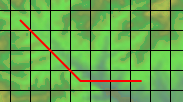
\includegraphics{diagonalpath}} 
\smallskip
    
Ścieżka ta ma \texttt{6} kwadratów szerokości i \texttt{3} kwadraty wysokości, a więc wykonujemy \texttt{6 - 3 = 3} prostych ruchów i \texttt{3} skośne.

    
Moglibyśmy odległość między dwoma punktami obliczać przy użyciu funkcji implementującej twierdzenie Pitagorasa. Potrzebujemy optymistycznego szacunku, a przyjęcie założenia, że można iść prosto do celu na pewno jest optymistyczne. Jednak im szacunek jest bliższy rzeczywistej odległości, tym mniej bezużytecznych ścieżek program musi sprawdzić.

  
\subsection*{Ćwiczenie 7.6}
\label{sol:7.6}
    
Jednym z dobrych pomysłów może być użycie obiektu zawierającego obiekty. Jedna ze współrzędnych punktów, np. \texttt{x}, jest używana jako nazwa własności dla zewnętrznego obiektu, a druga, \texttt{y}, dla obiektu wewnętrznego. To wymaga jednak prowadzenia zapisów, ponieważ czasami szukany obiekt wewnętrzny jeszcze nie będzie istniał.
    
\begin{verbatim} 
function makeReachedList() {
  return {};
}

function storeReached(list, point, route) {
  var inner = list[point.x];
  if (inner == undefined) {
    inner = {};
    list[point.x] = inner;
  }
  inner[point.y] = route;
}

function findReached(list, point) {
  var inner = list[point.x];
  if (inner == undefined)
    return undefined;
  else
    return inner[point.y];
}
\end{verbatim}
    
Inną możliwością jest połączenie współrzędnych \texttt{x} i \texttt{y} punktu w jedną nazwę własności i użycie jej do przechowywania tras w pojedynczym obiekcie.
    
\begin{verbatim} 
function pointID(point) {
  return point.x + "-" + point.y;
}

function makeReachedList() {
  return {};
}

function storeReached(list, point, route) {
  list[pointID(point)] = route;
}

function findReached(list, point) {
  return list[pointID(point)];
}
\end{verbatim}

\section*{Rozdział 8}
\label{sol:8}

\subsection*{Ćwiczenie 8.1}
\label{sol:8.1}
    
\begin{verbatim} 
function Point(x, y) {
  this.x = x;
  this.y = y;
}
Point.prototype.add = function(other) {
  return new Point(this.x + other.x, this.y + other.y);
};
Point.prototype.isEqualTo = function(other) {
  return this.x == other.x && this.y == other.y;
};

show((new Point(3, 1)).add(new Point(2, 4)));
\end{verbatim}
    
Pamiętaj, aby Twoja wersja metody \texttt{add} pozostawiała punkt \texttt{this} nietknięty i tworzyła nowy obiekt. Metoda zmieniająca bieżący obiekt działałaby podobnie do operatora \texttt{+=}, który z kolei działa jak operator \texttt{+}.

  
\subsection*{Ćwiczenie 8.2}
\label{sol:8.2}
    
\begin{verbatim} 
Grid.prototype.each = function(action) {
  for (var y = 0; y < this.height; y++) {
    for (var x = 0; x < this.width; x++) {
      var point = new Point(x, y);
      action(point, this.valueAt(point));
    }
  }
};
\end{verbatim}
  
 
\subsection*{Ćwiczenie 8.3}
\label{sol:8.3}
    
\begin{verbatim} 
Terrarium.prototype.toString = function() {
  var characters = [];
  var endOfLine = this.grid.width - 1;
  this.grid.each(function(point, value) {
    characters.push(characterFromElement(value));
    if (point.x == endOfLine)
      characters.push("\n");
  });
  return characters.join("");
};
 \end{verbatim}
    
Wypróbuj ten kod…

    
\begin{verbatim} 
var terrarium = new Terrarium(thePlan);
print(terrarium.toString());
// → ############################
//   #      #    #      o      ##
//   #                          #
//   #          #####           #
//   ##         #   #    ##     #
//   ###           ##     #     #
//   #           ###      #     #
//   #   ####                   #
//   #   ##       o             #
//   # o  #         o       ### #
//   #    #                     #
//   ############################
\end{verbatim}

  
\subsection*{Ćwiczenie 8.4}
\label{sol:8.4}
    
Nazwę metody można przekazać jako łańcuch. Dzięki temu funkcja \texttt{method} może sama znaleźć odpowiednią wartość funkcyjną.

    
\begin{verbatim} 
function method(object, name) {
  return function() {
    object[name].apply(object, arguments);
  };
}

var pushTest = method(testArray, "push");
\end{verbatim}

  
\subsection*{Ćwiczenie 8.5}
\label{sol:8.5}
    
\begin{verbatim} 
Terrarium.prototype.listSurroundings = function(center) {
  var result = {};
  var grid = this.grid;
  directions.each(function(name, direction) {
    var place = center.add(direction);
    if (grid.isInside(place))
      result[name] = characterFromElement(grid.valueAt(place));
    else
      result[name] = "#";
  });
  return result;
};
\end{verbatim}
    
Zwróć uwagę na użycie zmiennej \texttt{grid} w celu obejścia problemu z \texttt{this}.

  
\subsection*{Ćwiczenie 8.6}
\label{sol:8.6}
    
Aby wybrać losowy kierunek, potrzebna nam jest tablica nazw kierunków. Oczywiście moglibyśmy po prostu napisać \texttt{["n", "ne", ...]}, ale to oznaczałoby duplikowanie informacji, a powielanie danych mnie złości. Moglibyśmy też do budowy tej tablicy użyć instrukcji \texttt{each} w obiekcie \texttt{directions}, co byłoby już lepszym rozwiązaniem.
    
Jednak w tym przypadku jest możliwość zastosowania uogólnienia. Możliwość utworzenia listy nazw własności znajdujących się w słowniku wydaje się bardzo przydatna, a więc dodamy takie narzędzie do prototypu \texttt{Dictionary}.
    
\begin{verbatim} 
Dictionary.prototype.names = function() {
  var names = [];
  this.each(function(name, value) {names.push(name);});
  return names;
};

show(directions.names());
\end{verbatim}
    
Neurotyk od razu dodałby jeszcze dla równowagi metodę \texttt{values} zwracającą listę wartości zapisanych w słowniku. Myślę jednak, że to może poczekać, aż \href{http://www.c2.com/cgi/wiki?YouArentGonnaNeedIt}{będzie potrzebne}.
    
Oto sposób pobrania losowego elementu z tablicy:
    
\begin{verbatim} 
function randomElement(array) {
  if (array.length == 0)
    throw new Error("Tablica jest pusta.");
  return array[Math.floor(Math.random() * array.length)];
}

show(randomElement(["heads", "tails"]));
 \end{verbatim}
    
A to jest owad we własnej osobie:
    
\begin{verbatim} 
function DrunkBug() {};
DrunkBug.prototype.act = function(surroundings) {
  return {type: "move",
          direction: randomElement(directions.names())};
};
DrunkBug.prototype.character = "~";

creatureTypes.register(DrunkBug);
\end{verbatim}

  
\subsection*{Ćwiczenie 8.7}
\label{sol:8.7}
     
\begin{verbatim} 
function LichenEater() {
  this.energy = 10;
}
LichenEater.prototype.act = function(surroundings) {
  var emptySpace = findDirections(surroundings, " ");
  var lichen = findDirections(surroundings, "*");

  if (this.energy >= 30 && emptySpace.length > 0)
    return {type: "reproduce", direction: randomElement(emptySpace)};
  else if (lichen.length > 0)
    return {type: "eat", direction: randomElement(lichen)};
  else if (emptySpace.length > 0)
    return {type: "move", direction: randomElement(emptySpace)};
  else
    return {type: "wait"};
};
LichenEater.prototype.character = "c";

creatureTypes.register(LichenEater);
\end{verbatim}

  
\subsection*{Ćwiczenie 8.8}
\label{sol:8.8}
    
Jednym z rozwiązań może być rezygnacja z losowego wybierania kierunków ruchu. gdy kierunki są wybierane losowo, stwory często poruszają się w tę i~z~powrotem ostatecznie nigdzie nie docierając. Jeśli stworzenie będzie pamiętać kierunek ostatniego ruchu i preferować jego kontynuację, zmarnuje mniej czasu i szybciej dotrze do pożywienia.

    
\begin{verbatim} 
function CleverLichenEater() {
  this.energy = 10;
  this.direction = "ne";
}
CleverLichenEater.prototype.act = function(surroundings) {
  var emptySpace = findDirections(surroundings, " ");
  var lichen = findDirections(surroundings, "*");

  if (this.energy >= 30 && emptySpace.length > 0) {
    return {type: "reproduce",
            direction: randomElement(emptySpace)};
  }
  else if (lichen.length > 1) {
    return {type: "eat",
            direction: randomElement(lichen)};
  }
  else if (emptySpace.length > 0) {
    if (surroundings[this.direction] != " ")
      this.direction = randomElement(emptySpace);
    return {type: "move",
            direction: this.direction};
  }
  else {
    return {type: "wait"};
  }
};
CleverLichenEater.prototype.character = "c";

creatureTypes.register(CleverLichenEater);
 \end{verbatim}
    
Wypróbuj to na poprzedniej planszy terrarium.

  
\subsection*{Ćwiczenie 8.9}
\label{sol:8.9}
    
Rozwiązanie tego problemu musisz znaleźć sam. Mnie nie udało się znaleźć dobrego sposobu na to, aby zapobiec wyginięciu tych stworzeń natychmiast albo zaraz po wytępieniu wszystkich zjadaczy porostów. Sztuczka ze zjadaniem osobników tylko wtedy, gdy dwa z nich znajdują się obok siebie tutaj nie działa, ponieważ osobniki te się ruszają i trudno napotkać je, gdy są obok siebie. Obiecującym rozwiązaniem jest danie zjadaczom zjadaczy dużo energii, dzięki której mogą przetrwać czas, gdy jest mało zjadaczy porostów oraz powolne rozmnażanie, dzięki czemu zasoby pożywienia nie są zbyt szybko zużywane.

    
Życiem porostów i zjadaczy rządzi pewien cykl — raz jest dużo porostów, co powoduje, że rodzi się dużo zjadaczy, co z kolei powoduje, że robi się mało porostów, z którego to powodu zjadacze zaczynają umierać z głodu, co sprawia że porosty znowu się rozrastają itd. Można też spróbować hibernacji zjadaczy zjadaczy porostów (przy użyciu akcji \texttt{wait}) na pewien czas, gdy nie uda im się znaleźć nic do jedzenia przez kilka kolejek. Dobre efekty może przynieść wybudzanie stworów z hibernacji po odpowiedniej liczbie kolejek albo gdy wyczują w pobliżu jedzenie.

\section*{Rozdział 10}
\label{sol:10}

\subsection*{Ćwiczenie 10.1}
\label{sol:10.1}
    
\begin{verbatim} 
var datePattern = /\d\d\/\d\d\/\d\d\d\d/;
show("urodzeni 15/11/2003 (matka Spot): White Fang".search(datePattern));
\end{verbatim}
 
  
\subsection*{Ćwiczenie 10.2}
\label{sol:10.2}
    
\begin{verbatim} 
var mailAddress = /\b[\w\.-]+@[\w\.-]+\.\w{2,3}\b/;

show(mailAddress.test("kenny@test.net"));
show(mailAddress.test("Wyłsałem mleja na adres kenny@tets.nets, ale nie dźła!"));
show(mailAddress.test("the_giant_sloth@gmail.com"));
 \end{verbatim}
    
Ciągi \texttt{\textbackslash b} na początku i końcu wzorca sprawiają, że drugi łańcuch nie pasuje.

  
\subsection*{Ćwiczenie 10.3}
\label{sol:10.3}
    
\begin{verbatim} 
function extractDate(string) {
  var found = string.match(/(\d\d?)\.(\d\d?)\.(\d{4})/);
  if (found == null)
    throw new Error("Nie znaleziono daty w „" + string + "”.");
  return new Date(Number(found[3]), Number(found[2]) - 1,
                  Number(found[1]));
}

show(extractDate("urodzeni 5.2.2007 (matka Noog): Long-ear Johnson"));
\end{verbatim}
    
Ta wersja jest nieco dłuższa niż poprzednia, ale ma tę zaletę, że sprawdza co robi i złości się, gdy otrzyma bezsensowne dane. Bez wyrażeń regularnych osiągnięcie tego było dużo trudniejsze ― trzeba by było wykonać wielu wywołań funkcji \texttt{indexOf}, aby dowiedzieć się czy liczby zawierają jedną cyfrę czy dwie oraz czy łączniki znajdowały się we właściwych miejscach.

  
\subsection*{Ćwiczenie 10.4}
\label{sol:10.4}
    
\begin{verbatim} 
function escapeHTML(text) {
  var replacements = {"<": "<", ">": ">",
                      "&": "&", "\"": """};
  return text.replace(/[<>&"]/g, function(character) {
    return replacements[character];
  });
}

print(escapeHTML("Tekst preformatowany zapisuje się w elemencie \"<pre>\"."));
\end{verbatim}
    
Obiekt \texttt{replacements} pozwala szybko związać każdy znak z jego encją. Używanie go w ten sposób jest bezpieczne (tzn. nie jest potrzebny żaden obiekt \texttt{Dictionary}), ponieważ jedyne własności, jakie będą używane to te, które zostaną dopasowane przez wyrażenie \texttt{/[<>\&"]/}.

\section*{Rozdział 11}
\label{sol:11}
  
\subsection*{Ćwiczenie 11.1}
\label{sol:11.1}
    
\begin{verbatim} 
function validInfo(form) {
  return form.elements.name.value != "" &&
    /^.+@.+\.\w{2,3}$/.test(form.elements.email.value);
}

show(validInfo(document.forms.userinfo));
\end{verbatim}
    
Gdy zastanawiałeś się nad sprawdzaniem adresu e-mail, przyszło ci do głowy, aby użyć wyrażeń regularnych, prawda?

  
\subsection*{Ćwiczenie 11.2}
\label{sol:11.2}
    
\begin{verbatim} 
userForm.elements.send.onclick = function() {
  if (validInfo(userForm))
    userForm.submit();
  else
    alert("Podaj nazwisko i poprawny adres e-mail!");
};
\end{verbatim}

\section*{Rozdział 12}
\label{sol:12}

\subsection*{Ćwiczenie 12.1}
\label{sol:12.1}
     
\begin{verbatim} 
function asHTML(node) {
  if (isTextNode(node))
    return escapeHTML(node.nodeValue);
  else if (node.childNodes.length == 0)
    return "<" + node.nodeName + "/>";
  else
    return "<" + node.nodeName + ">" +
           map(asHTML, node.childNodes).join("") +
           "</" + node.nodeName + ">";
}

print(asHTML(document.body));
\end{verbatim}

  
\subsection*{Ćwiczenie 12.2}
\label{sol:12.2}
    
\begin{verbatim} 
function removeElement(node) {
  if (node.parentNode)
    node.parentNode.removeChild(node);
}

removeElement(newParagraph);
\end{verbatim}
  
  
\subsection*{Ćwiczenie 12.3}
\label{sol:12.3}
    
\begin{verbatim} 
function makeTable(data, columns) {
  var headRow = dom("TR");
  forEach(columns, function(name) {
    headRow.appendChild(dom("TH", null, name));
  });

  var body = dom("TBODY", null, headRow);
  forEach(data, function(object) {
    var row = dom("TR");
    forEach(columns, function(name) {
      row.appendChild(dom("TD", null, String(object[name])));
    });
    body.appendChild(row);
  });

  return dom("TABLE", null, body);
}

var table = makeTable(document.body.childNodes,
                      ["nodeType", "tagName"]);
document.body.appendChild(table);
\end{verbatim}
    
Nie zapomnij przekonwertować wartości z obiektów na łańcuchy przed ich dodaniem do tabeli ― nasza funkcja \texttt{dom} rozpoznaje tylko łańcuchy i węzły DOM.


\section*{Rozdział 13}
\label{sol:13}
 
\subsection*{Ćwiczenie 13.1}
\label{sol:13.1}   
    
\begin{verbatim} 
function registerEventHandler(node, event, handler) {
  if (typeof node.addEventListener == "function")
    node.addEventListener(event, handler, false);
  else
    node.attachEvent("on" + event, handler);
}

registerEventHandler($("button"), "click",
                     function(){print("Klik (2)");});
\end{verbatim}
    
Nie przestrasz się tej długiej i niezgrabnej nazwy. Później będziemy musieli dodać nowe opakowanie, aby opakować to opakowanie i będzie ono miało krótszą nazwę.

    
Można też test ten wykonać tylko raz i zdefiniować \texttt{registerEventHandler} do przechowywania innej funkcji w zależności od przeglądarki. Takie rozwiązanie jest lepsze pod względem wydajnościowym, ale trochę dziwne.

    
\begin{verbatim} 
if (typeof document.addEventListener == "function")
  var registerEventHandler = function(node, event, handler) {
    node.addEventListener(event, handler, false);
  };
else
  var registerEventHandler = function(node, event, handler) {
    node.attachEvent("on" + event, handler);
  };
\end{verbatim}

  
\subsection*{Ćwiczenie 13.2}
\label{sol:13.2}
 
    
\begin{verbatim} 
Square.moveContent = function(target) {
  target.content = this.content;
  this.content = null;
  target.tableCell.appendChild(this.tableCell.lastChild);
};
Square.clearContent = function() {
  this.content = null;
  removeElement(this.tableCell.lastChild);
};
 \end{verbatim}
  
  
\subsection*{Ćwiczenie 13.3}
\label{sol:13.3}
      
\begin{verbatim} 
SokobanField.move = function(direction) {
  var playerSquare = this.getSquare(this.playerPos);
  var targetPos = this.playerPos.add(direction);
  var targetSquare = this.getSquare(targetPos);

  // Możliwość przesunięcia kamienia
  if (targetSquare.hasBoulder()) {
    var pushTarget = this.getSquare(targetPos.add(direction));
    if (pushTarget.isEmpty()) {
      targetSquare.moveContent(pushTarget);
    }
    else if (pushTarget.isExit()) {
      targetSquare.moveContent(pushTarget);
      pushTarget.clearContent();
      this.bouldersToGo--;
      this.updateScore();
    }
  }
  // Przesuwanie gracza
  if (targetSquare.isEmpty()) {
    playerSquare.moveContent(targetSquare);
    this.playerPos = targetPos;
  }
};
\end{verbatim}
    
Dzięki temu, że najpierw obsługiwany jest ruch kamieni, kod ruchu może działać w taki sam sposób zarówno gdy gracz przesuwa się normalnie, jak i gdy popycha kamień. Zwróć uwagę na sposób zlokalizowania kwadratu za kamieniem poprzez dodanie \texttt{direction} dwa razy do \texttt{playerPos}. Przetestuj ten kod przesuwając się w lewo o dwa kwadraty:
    
\begin{verbatim} 
testField.move(new Point(-1, 0));
testField.move(new Point(-1, 0));
\end{verbatim}
    
Jeśli to zadziałało, to przesunęliśmy kamień w miejsce, z którego nie da się go już ruszyć, a więc lepiej to pole usunąć.
    
\begin{verbatim} 
testField.remove();
\end{verbatim}

  
\subsection*{Ćwiczenie 13.4}
\label{sol:13.4}
    
\begin{verbatim} 
SokobanGame.keyDown = function(event) {
  if (arrowKeyCodes.contains(event.keyCode)) {
    event.stop();
    this.field.move(arrowKeyCodes.lookup(event.keyCode));
    if (this.field.won()) {
      if (this.level < sokobanLevels.length - 1) {
        alert("Doskonale! Przechodzisz do następnego poziomu.");
        this.level++;
        this.reset();
      }
      else {
        alert("Wygrałeś! Koniec gry.");
        this.newGame();
      }
    }
  }
};
\end{verbatim}
    
Należy zaznaczyć, że taki sposób przechwytywania zdarzeń klawiszy ― poprzez dodanie procedury do \texttt{document} i zatrzymywanie tych zdarzeń, które nas interesują — nie jest dobrym pomysłem, jeśli w dokumencie znajdują się inne elementy. Spróbuj na przykład przesunąć kursor w polu tekstowym znajdującym się na górze dokumentu. ― Nie uda Ci się to, ponieważ przesuniesz tylko ludzika w grze Sokoban. Gdyby gra miała być używana na prawdziwej stronie internetowej, najlepiej byłoby ją umieścić w ramce lub osobnym oknie, aby przejmowała tylko zdarzenia dotyczące niej.

  
\subsection*{Ćwiczenie 13.5}
\label{sol:13.5}   
    
Czas animacji można kontrolować za pomocą metody \texttt{setInterval}. Pamiętaj,że metoda ta powinna się wyłączyć po wykonaniu swojego zadania. Jeśli tego nie zrobisz, będzie marnowała zasoby komputera dopóki strona nie zostanie zamknięta.

    
\begin{verbatim} 
Square.clearContent = function() {
  self.content = null;
  var image = this.tableCell.lastChild;
  var size = 100;

  var animate = setInterval(function() {
    size -= 10;
    image.style.width = size + "%";
    image.style.height = size + "%";

    if (size < 60) {
      clearInterval(animate);
      removeElement(image);
    }
  }, 70);
};
\end{verbatim}
    
Teraz, jeśli masz kilka godzin możesz spróbować przejść wszystkie poziomy.


\section*{Rozdział 14}
\label{sol:14}

\subsection*{Ćwiczenie 14.1}
\label{sol:14.1}
    
\begin{verbatim} 
function serializeJSON(value) {
  function isArray(value) {
    return /^\s*function Array/.test(String(value.constructor));
  }

  function serializeArray(value) {
    return "[" + map(serializeJSON, value).join(", ") + "]";
  }
  function serializeObject(value) {
    var properties = [];
    forEachIn(value, function(name, value) {
      properties.push(serializeString(name) + ": " +
                      serializeJSON(value));
    });
    return "{" + properties.join(", ") + "}";
  }
  function serializeString(value) {
    var special =
      {"\"": "\\\"", "\\": "\\\\", "\f": "\\f", "\b": "\\b",
       "\n": "\\n", "\t": "\\t", "\r": "\\r", "\v": "\\v"};
    var escaped = value.replace(/[\"\\\f\b\n\t\r\v]/g,
                                function(c) {return special[c];});
    return "\"" + escaped + "\"";
  }

  var type = typeof value;
  if (type == "object" && isArray(value))
    return serializeArray(value);
  else if (type == "object")
    return serializeObject(value);
  else if (type == "string")
    return serializeString(value);
  else
    return String(value);
}

print(serializeJSON(fruit));
\end{verbatim}
    
Sztuczka użyta w funkcji \texttt{serializeString} jest podobna do tego, co zrobiliśmy w funkcji \texttt{escapeHTML} w \hyperref[chap:10]{rozdziale 10}. Zastępnik dla każdego znaku jest znajdowany w obiekcie. Niektóre z nich, jak choćby \texttt{"\textbackslash \textbackslash \textbackslash \textbackslash"}, wyglądają dziwnie, ponieważ każdy ukośnik wsteczny, który ma się pojawić w wyniku musi mieć towarzyszący ukośnik wsteczny.

    
Zwróć też uwagę, że także nazwy własności są zapisane w cudzysłowach, jako łańcuchy. W niektórych przypadkach nie jest to konieczne, ale dla nazw zawierających spacje i jakieś inne dziwne rzeczy tak. Tu zostało użyte uproszczone rozwiązanie polegające na ujęciu w cudzysłów wszystkiego.
